% Copyright 2021  Ed Bueler

\documentclass[10pt,hyperref,dvipsnames]{beamer}

\mode<presentation>{
  \usetheme{Madrid}
  \usecolortheme{beaver}
  \setbeamercovered{transparent}
  \setbeamerfont{frametitle}{size=\large}
}

\setbeamercolor*{block title}{bg=red!10}
\setbeamercolor*{block body}{bg=red!5}

\usepackage[english]{babel}
\usepackage[latin1]{inputenc}
\usepackage{times}
\usepackage[T1]{fontenc}
% Or whatever. Note that the encoding and the font should match. If T1
% does not look nice, try deleting the line with the fontenc.

\usepackage{empheq}
\usepackage{xspace}
\usepackage{verbatim,fancyvrb}

\usepackage{tikz}
\usetikzlibrary{shapes,arrows.meta,decorations.markings,decorations.pathreplacing,fadings,positioning}

\usepackage{hyperref}

% If you wish to uncover everything in a step-wise fashion, uncomment
% the following command:
%\beamerdefaultoverlayspecification{<+->}

\newcommand{\ba}{\mathbf{a}}
\newcommand{\bb}{\mathbf{b}}
\newcommand{\bc}{\mathbf{c}}
\newcommand{\bbf}{\mathbf{f}}
\newcommand{\bg}{\mathbf{g}}
\newcommand{\bn}{\mathbf{n}}
\newcommand{\bq}{\mathbf{q}}
\newcommand{\br}{\mathbf{r}}
\newcommand{\bx}{\mathbf{x}}
\newcommand{\by}{\mathbf{y}}
\newcommand{\bv}{\mathbf{v}}
\newcommand{\bu}{\mathbf{u}}
\newcommand{\bw}{\mathbf{w}}

\newcommand{\bF}{\mathbf{F}}
\newcommand{\bG}{\mathbf{G}}
\newcommand{\bQ}{\mathbf{Q}}

\newcommand{\bzero}{\mathbf{0}}

\newcommand{\grad}{\nabla}
\newcommand{\Div}{\nabla\cdot}
\newcommand{\minmod}{\operatorname{minmod}}

\newcommand{\CC}{\mathbb{C}}
\newcommand{\RR}{\mathbb{R}}

\newcommand{\ddt}[1]{\ensuremath{\frac{\partial #1}{\partial t}}}
\newcommand{\ddx}[1]{\ensuremath{\frac{\partial #1}{\partial x}}}
\newcommand{\Matlab}{\textsc{Matlab}\xspace}
\newcommand{\Octave}{\textsc{Octave}\xspace}
\newcommand{\eps}{\epsilon}

\newcommand{\ip}[2]{\left<#1,#2\right>}

\newcommand{\trefcolumn}[1]{\begin{bmatrix} \phantom{x} \\ #1 \\ \phantom{x} \end{bmatrix}}
\newcommand{\trefmatrixtwo}[2]{\left[\begin{array}{c|c|c} & & \\ #1 & \dots & #2 \\ & & \end{array}\right]}
\newcommand{\trefmatrixthree}[3]{\left[\begin{array}{c|c|c|c} & & & \\ #1 & #2 & \dots & #3 \\ & & & \end{array}\right]}
\newcommand{\trefmatrixgroups}[4]{\left[\begin{array}{c|c|c|c|c|c} & & & & & \\ #1 & \dots & #2 & #3 & \dots & #4 \\ & & & & & \end{array}\right]}

\newcommand{\blocktwo}[4]{\left[\begin{array}{c|c} #1 & #2 \\ \hline #3 & #4 \end{array}\right]}

\newcommand{\ds}{\displaystyle}


\title{Stokes problems using Firedrake}

\subtitle{A glacier and ice sheet tutorial}

\author{Ed Bueler}

\institute[UAF]{University of Alaska Fairbanks}

\date[April 2021]{April 2021  \\ \phantom{foo} \\ \phantom{foo} \\
\large \href{https://github.com/bueler/stokes-ice-tutorial}{\alert{\texttt{github.com/bueler/stokes-ice-tutorial}}} }


\begin{document}
\beamertemplatenavigationsymbolsempty

\begin{frame}
  \maketitle
\end{frame}

\begin{frame}
  \frametitle{Outline}

\centerline{\large \href{https://github.com/bueler/stokes-ice-tutorial}{\alert{\texttt{github.com/bueler/stokes-ice-tutorial}}}}

\bigskip
  \tableofcontents[hideallsubsections]
\end{frame}


\section{the problem}

\begin{frame}{the glacier dynamics problem}

\begin{itemize}
\item FIXME show results on velocity and pressure
\item \alert{there is a lot I cannot explain in an hour, so please try the codes and send questions by email!}
\end{itemize}
\end{frame}

\section{the equations}

\newcommand{\rhoi}{\rho_{\text{i}}}
\begin{frame}{Glen-Stokes equations}

\begin{columns}
\begin{column}{0.8\textwidth}
\begin{align*}
- \nabla \cdot \tau + \nabla p &= \rhoi \bg &&\text{\emph{stress balance}} \\
\nabla \cdot \bu &= 0 &&\text{\emph{incompressibility}} \\
\tau &= B_n |D\bu|^{(1/n) - 1} D\bu  &&\text{\emph{Glen flow law}}
\end{align*}
\end{column}

\begin{column}{0.2\textwidth}

\vspace{5mm}
%https://www.bl.uk/voices-of-science/interviewees/john-glen#
\hfill 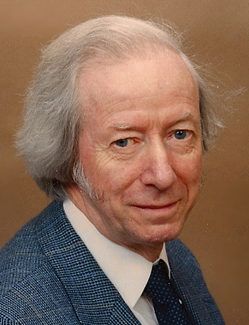
\includegraphics[width=0.6\textwidth]{figs/people/jglen.png}
\end{column}
\end{columns}

\bigskip
\begin{itemize}
\item constants: {\small $\rhoi=910 \,\text{kg}\,\text{m}^{-3}$, $g=9.81\,\text{m}\,\text{s}^{-2}$, $n=3$, $B_n=6.8\times 10^7\,\text{Pa}\,\text{s}^{1/3}$}
\item viscosity regularization with $\eps = 10^{-4}$ and $D_0 = 1\,\text{a}^{-1}$:
\begin{equation*}
\nu_\eps(|D\bu|) = \frac{1}{2} B_n \left(|D\bu|^2 + \eps\, D_0^2\right)^{((1/n) - 1)/2}
\end{equation*}
\item eliminate $\tau$ to give system for $\bu,p$:
\begin{align*}
- \nabla \cdot \left(2 \nu_\eps(|D\bu|)\, D\bu\right) + \nabla p &= \rhoi \mathbf{g} \\
\Div \bu &= 0
\end{align*}
\end{itemize}
\end{frame}

\section{\texttt{stage1/} \qquad linear Stokes}

\begin{frame}{the linear Stokes equations}

\begin{columns}

\begin{column}{0.6\textwidth}
\begin{itemize}
\item if we make viscosity constant ($\nu_0$) then we get the linear Stokes system:
\begin{align*}
- \nabla \cdot \left(2 \nu_0\, D\bu\right) + \nabla p &= \rhoi \mathbf{g}  \\
\Div \bu &= 0
\end{align*}
\item with reformatting:
\begin{align*}
- \nu_0 \nabla^2 \bu + \nabla p &= \rhoi \mathbf{g}  \\
-\Div \bu \qquad \,\,\,\, &= 0
\end{align*}
\item it has symmetric block structure
  $$\begin{bmatrix} A & B^\top \\ B & 0 \end{bmatrix} \begin{bmatrix} \bu \\ p  \end{bmatrix} = \begin{bmatrix} \bbf \\ 0 \end{bmatrix}$$
\end{itemize}
\end{column}

\begin{column}{0.4\textwidth}
\hfill 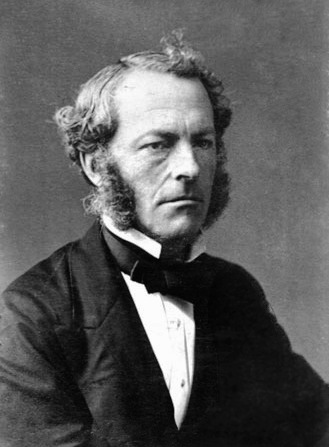
\includegraphics[width=0.4\textwidth]{figs/people/gstokes.jpg}

\vspace{10mm}
\hfill 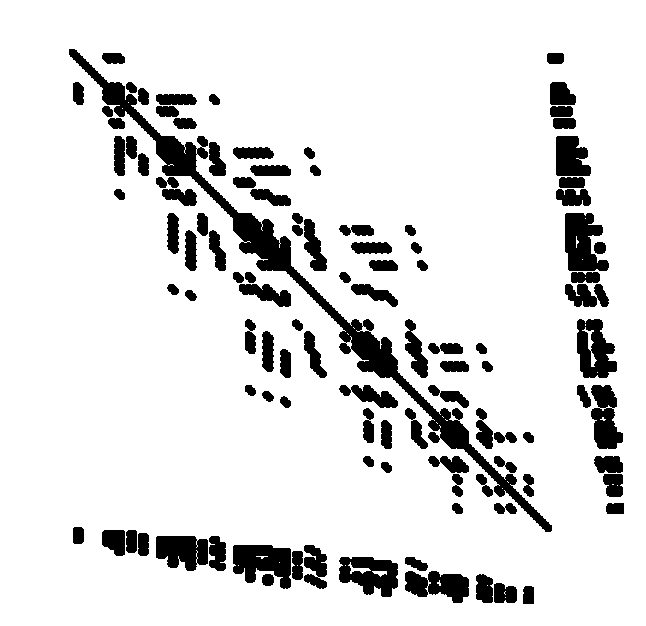
\includegraphics[width=0.8\textwidth]{figs/Kstokes.pdf}
\end{column}

\end{columns}
\end{frame}


\begin{frame}{boundary conditions}

\begin{itemize}
\item stress-free top:
\begin{equation*}
\sigma \bn = \left(2 \nu_\eps(|D\bu|) D\bu - pI\right) \bn = \bzero
\end{equation*}
\item no slip base:
\begin{equation*}
\bu = \bzero
\end{equation*}
\end{itemize}
\end{frame}


\begin{frame}{finite elements}

\begin{itemize}
\item FIXME
\end{itemize}
\end{frame}


\begin{frame}[fragile]
\frametitle{weak form}

\begin{itemize}
\item FIXME
\item in the \texttt{stage1/} solver it looks like:
\begin{Verbatim}
    F = nu0 * inner(D(u), D(v)) * dx \
        - p * div(v) * dx \
        - div(u) * q * dx \
        - inner(fbody, v) * dx
\end{Verbatim}
\end{itemize}
\end{frame}


\begin{frame}[fragile]
\frametitle{activate the virtual environment}

\begin{itemize}
\item before using Firedrake you always need to activate the Python \texttt{venv}
\item I have an alias \texttt{drakeme} for this
\end{itemize}

\bigskip
\begin{Verbatim}
$ unset PETSC_DIR; unset PETSC_ARCH;  # may be needed
$ source ~/firedrake/bin/activate
\end{Verbatim}
\end{frame}


\begin{frame}[fragile]
\frametitle{\texttt{stage1/} \qquad linear Stokes}

\begin{itemize}
\item \emph{purpose:} solve linear Stokes on a trapezoidal glacier
\item \emph{source files:} \texttt{domain.geo}, \texttt{solve.py} \hfill \alert{$\gets$ inspect these!}
\item \emph{generated files:} \texttt{domain.msh}, \texttt{domain\_0.vtu}, \texttt{domain.pvd}
\end{itemize}

\bigskip
\begin{Verbatim}
$ cd stage1/
$ gmsh -2 domain.geo                  # mesh domain
$ gmsh domain.msh                     # view mesh
$ ./solve.py                          # solve Stokes
$ paraview domain.pvd                 # view solution
\end{Verbatim}
%$

\vspace{10mm}
\begin{center}

\includegraphics[width=0.9\textwidth]{figs/stage1.png}
\end{center}
\end{frame}


\section{\texttt{stage2/} \qquad Glen-Stokes}

\begin{frame}{Newton's method}

\hfill 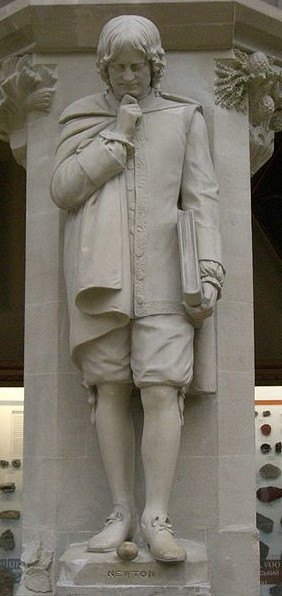
\includegraphics[width=0.2\textwidth]{figs/people/inewton.jpg}

\vspace{-20mm}
\begin{itemize}
\item FIXME
\end{itemize}
\end{frame}


\begin{frame}[fragile]
\frametitle{\texttt{stage2/} \qquad Glen-Stokes}

\begin{itemize}
\item \emph{purpose:} solve Glen-Stokes on a flat-bed glacier
\item \emph{source files:} \texttt{domain.py}, \texttt{solve.py} \hfill \alert{$\gets$ inspect these!}
\item \emph{generated files:} \texttt{dome.geo}, \texttt{dome.msh}, \texttt{dome\_0.vtu}, \texttt{dome.pvd}
\end{itemize}

\bigskip
\begin{Verbatim}
$ cd stage2/
$ ./domain.py                   # generate geometry
$ gmsh -2 dome.geo              # mesh domain
$ gmsh dome.msh                 # view mesh
$ ./solve.py -s_snes_monitor -s_snes_converged_reason
$ paraview dome.pvd             # view solution
\end{Verbatim}

\vspace{10mm}
\begin{center}
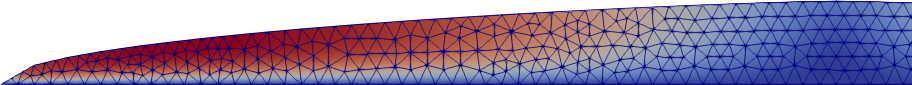
\includegraphics[width=0.9\textwidth]{figs/stage2.png}
\end{center}
\end{frame}


\section{\texttt{stage3/} \qquad extruded meshes}

\begin{frame}[fragile]
\frametitle{\texttt{stage3/} \qquad extruded meshes}

\begin{itemize}
\item \emph{purpose:} solve same problem using an extruded quadrilateral mesh
\item \emph{source files:} \texttt{solve.py} \hfill \alert{$\gets$ inspect this!}
\item \emph{generated files:} \texttt{dome\_0.vtu}, \texttt{dome.pvd}
\end{itemize}

\bigskip
\begin{Verbatim}
$ cd stage3/
$ ./solve.py -s_snes_monitor -s_snes_converged_reason
$ paraview dome.pvd
\end{Verbatim}
%$

\vspace{10mm}
\begin{center}
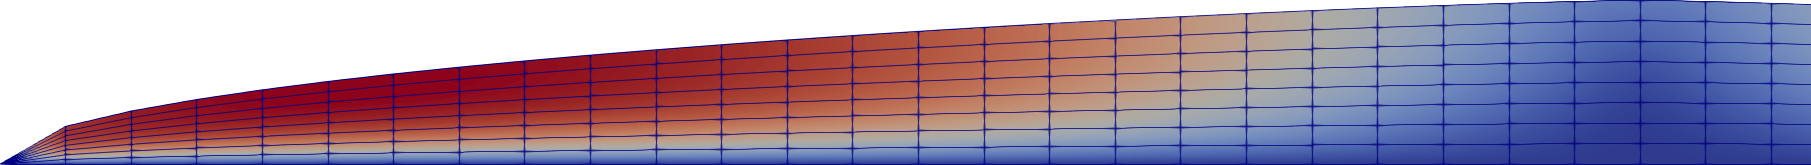
\includegraphics[width=0.9\textwidth]{figs/stage3.png}
\end{center}
\end{frame}


\begin{frame}[fragile]
\frametitle{convergence?}

% timer ./solve.py -s_snes_rtol 1.0e-5 -s_snes_max_it 200 -s_snes_converged_reason -mx MX -mz MZ
% timer ./solve.py -s_snes_rtol 1.0e-5 -s_snes_max_it 200 -s_snes_converged_reason -mx 640 -mz 64 -eps 0.01
\begin{center}
\begin{tabular}{c|rrr}
mesh           &   $\Delta x$ (m) & av.~speed & max.~speed \\ \hline
$20\times 2$   &             1000 &      1813 &       3512 \\
$40\times 4$   &              500 &      1787 &       3293 \\
$80\times 8$   &              250 &      1769 &       3223 \\
$160\times 16$ &              125 &      1762 &       3199 \\
$320\times 32$ &             62.5 &      1759 &       3191 \\
$640\times 64$ &            31.25 &      1758 &       3190
\end{tabular}
\end{center}

\begin{itemize}
\item \texttt{stage3/} code \texttt{solve.py} is set-up for adjustable resolution, e.g.:
\begin{Verbatim}
$ ./solve.py -mx 20 -mz 2
\end{Verbatim}
%$
\item results are reasonable and consistent
\item unfortunately the $640\times 64$ run needed $\eps=10^{-2}$ to get ``unstuck'' from the $\bu=0,p=0$ initial iterate
\end{itemize}
\end{frame}


\begin{frame}{performance?}

% same runs as above
% N = MX MZ (4*2 + 1)  is approximately correct for Q2xQ1
% SNES iterations: 92, 11, 13, 11, 15, 16
\begin{center}
\begin{tabular}{c|rr|rr}
mesh           &   $N$ & ratio & run time (s)  & ratio \\ \hline
$20\times 2$   &    360 &       &          2.0 &       \\
$40\times 4$   &   1440 &     4 &          1.9 &   1.0 \\
$80\times 8$   &   5760 &     4 &          2.5 &   1.3 \\
$160\times 16$ &  23040 &     4 &          5.7 &   2.3 \\
$320\times 32$ &  92160 &     4 &         31.9 &   5.6 \\
$640\times 64$ & 368640 &     4 &        255.9 &   8.0
\end{tabular}
\end{center}

\begin{itemize}
\item \texttt{stage3/} \texttt{solve.py} performance shown above
\item \emph{ideally}, if number of degrees of freedom $N$ increases by 4 then time should increase by 4
\item \alert{we need faster solvers and better initial iterates for high resolution and 3D solutions}
\end{itemize}
\end{frame}



\section{\texttt{stage4/} \qquad faster and finer}

\begin{frame}{iterative linear methods}

\hfill 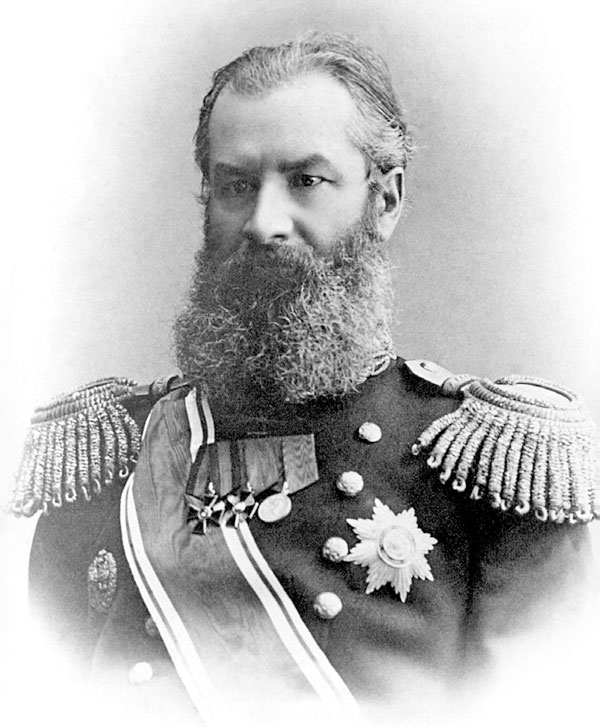
\includegraphics[width=0.2\textwidth]{figs/people/akrylov.jpg}

\vspace{-20mm}
\begin{itemize}
\item FIXME
\end{itemize}
\end{frame}

\begin{frame}{multigrid}

\hfill 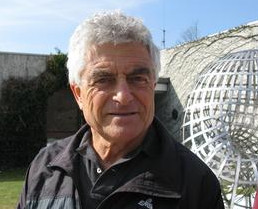
\includegraphics[width=0.25\textwidth]{figs/people/abrandt.jpg}

\vspace{-20mm}

\begin{itemize}
\item FIXME
\end{itemize}
\end{frame}


\section{\texttt{stage5/} \qquad 3D}

\begin{frame}{learn more}

\centerline{\large \href{https://github.com/bueler/stokes-ice-tutorial}{\alert{\texttt{github.com/bueler/stokes-ice-tutorial}}}}

\medskip
\hrulefill


\begin{columns}
\begin{column}{0.6\textwidth}
\small

\begin{itemize}
\item Firedrake: \href{https://www.firedrakeproject.org/}{\texttt{firedrakeproject.org}}

    \begin{itemize}
    \scriptsize
    \item tutorials \& manual: \href{https://www.firedrakeproject.org/documentation.html}{\texttt{.../documentation.html}}
    \item Jupyter notebooks page: \href{https://www.firedrakeproject.org/notebooks.html}{\texttt{.../notebooks.html}}
    \end{itemize}
\item PETSc website: \href{https://www.mcs.anl.gov/petsc/}{\texttt{www.mcs.anl.gov/petsc}}
\item for glacier Stokes eqns, see Ch.~1 by Hewitt:


{\scriptsize Fowler \& Ng, ed., \emph{Glaciers and Ice Sheets in the Climate System: The Karthaus Summer School Lecture Notes}, Springer 2021}

\item for finite elements and linear Stokes:

{\scriptsize Elman, Silvester, \& Wathen, \emph{Finite Elements and Fast Iterative Solvers, With Applications in Incompressible Fluid Dynamics}, Oxford 2014, 2nd ed.}

\item for PETSc, Firedrake, and Stokes (Ch.~14):

{\scriptsize Bueler, \emph{PETSc for Partial Differential Equations: Numerical Solutions in C and Python}, SIAM 2021}
\end{itemize}
\end{column}

\begin{column}{0.4\textwidth}

\bigskip
\href{https://www.firedrakeproject.org/}{
\includegraphics[width=\textwidth]{figs/firedrakebanner.png}}

\bigskip
\hfill \href{https://www.mcs.anl.gov/petsc/}{
\includegraphics[width=0.6\textwidth]{figs/petscbanner.png}}

\vspace{25mm}

\includegraphics[width=0.31\textwidth]{figs/covers/karthaus.png} \hfill
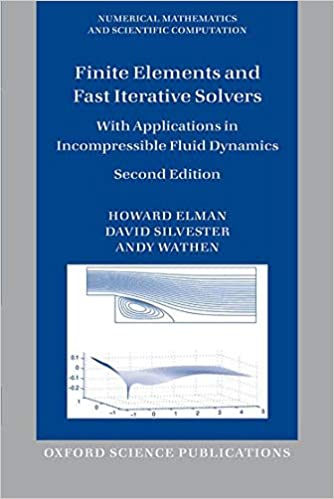
\includegraphics[width=0.31\textwidth]{figs/covers/elman.jpg} \hfill
\href{https://my.siam.org/Store/Product/viewproduct/?ProductId=32850137}{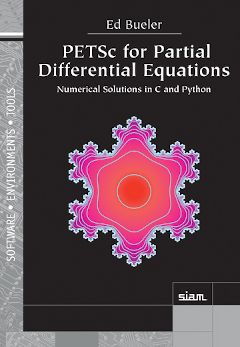
\includegraphics[width=0.32\textwidth]{figs/covers/bueler.jpg}}
\end{column}

\end{columns}
\end{frame}


\end{document}
